\begin{prp}[count=9] Soit une fonction affine $f\colon x\mapsto ax+b$.
\begin{itemize}
\item Si $a<0$ alors : \hspace*{0.5cm}
\begin{minipage}[c]{0.7\linewidth}
{\centering
\begin{tikzpicture}
\tkzTabInit[lgt=3,espcl=3]{$x$ /0.75%
				, signe de $f(x)$ /0.75}%
{$-\infty$,$\color{red}-\frac{b}{a}$,$+\infty$}%
\tkzTabLine{ , \color{red}+ , z ,\color{red}- , }
\end{tikzpicture}

} 
\end{minipage}
  \item Si $a>0$ alors : \hspace*{0.5cm}
\begin{minipage}[c]{0.7\linewidth}
{\centering
\begin{tikzpicture}
\tkzTabInit[lgt=3,espcl=3]{$x$ /0.75%
				, signe de $f(x)$ /0.75}%
{$-\infty$,$\color{red}-\frac{b}{a}$,$+\infty$}%
\tkzTabLine{ , \color{red}- , z , \color{red}+ , }%\noexpand\pointille{$-\frac{b}{a}$}
\end{tikzpicture}

}
\end{minipage}
\end{itemize}
\end{prp}

